\clearpage
\subsection{Vihreä nahkalilja 23.3.}

\begin{multicols}{2}

	Seitsemän rohkeaa rusakkoa, \mbox{Ahti}, Elias, Janne, Leo, Mikko,
	\mbox{Tanguy} ja Toivo, lähtivät uhmaamaan fyysistä ja henkistä kestävyyttään
	melkein keväisenä maaliskuun aamuna tavoitteenaan taittaa
	neljänkymmenen kilometrin matka vuorokaudessa – niin sanottu vihreä
	nahkalilja. Nahkaliljat ovat vyössä kannettavia partiomerkkejä, joiden
	tarkoituksena on tähdentää ulkoilun merkitystä ja innostaa partiolaisia
	ylläpitämään ja kehittämään peruskuntoaan. Rusakoissa tähdennys ja
	innostus on jäänyt viime vuosina vähemmälle, sillä edellisistä
	nahkaliljoista on ehtinyt vierähtää jo tovi: viimeksi nahkaliljoja on
	vaellettu 26.–27.10.2018, 8.–9.5.2015, 3.–4.5.2014 ja 4.–5.5.2013. Nyt
	kuitenkin innokas porukka on saatu kasaan ja reittimestari Ahti on
	suunnitellut käveltävän reitin Helsingin Mikaelinkirkolta ja takaisin
	paikoin Helsingin itäistä rantareittiä mukaillen – vähän niin kuin
	vuonna 2013, kun allekirjoittanut vaelsi Espoon Rantaraittia
	Kauklahdesta Helsingin keskustaan!

	Vaelluksen lähtö ja maali olivat Mikaelinkirkolla, jonne rusakot
	kokoontuivat aamuyhdeksäksi. Matkaan päästiin vasta \textbf{kello
	9.05}, koska seurue jäi odottamaan kahta nahkaliljaan ilmoittautunutta,
	jotka eivät kuitenkaan ilmestyneet lähtöön. Lähtöaika tarkistettiin
	reittimestarin kellosta ja merkittiin tarkasti muistiin. Niin ikään osa
	osallistujista käynnisti omat satelliitteihin tai muihin antureihin
	tukeutuvat matkamittarinsa, kun taas itse vaellusreitti oli
	perinteikkäästi piirretty karttatulosteelle.

	Liikkeelle lähdettiin kohti Emännänpuistoa ja alustavaksi
	taukostrategiaksi sovittiin, että viiden minuutin taukoja pidettäisiin
	aina viiden kilometrin välein. Harkittiinpa myös ajanvietteeksi laskea
	matkan aikana ylitettävät sillat, joista ensimmäiset tulivat vastaan
	varsin pian, kun ylitettiin Kontulantie ja metron raiteet.

	\vspace*{0.32cm}
	\noindent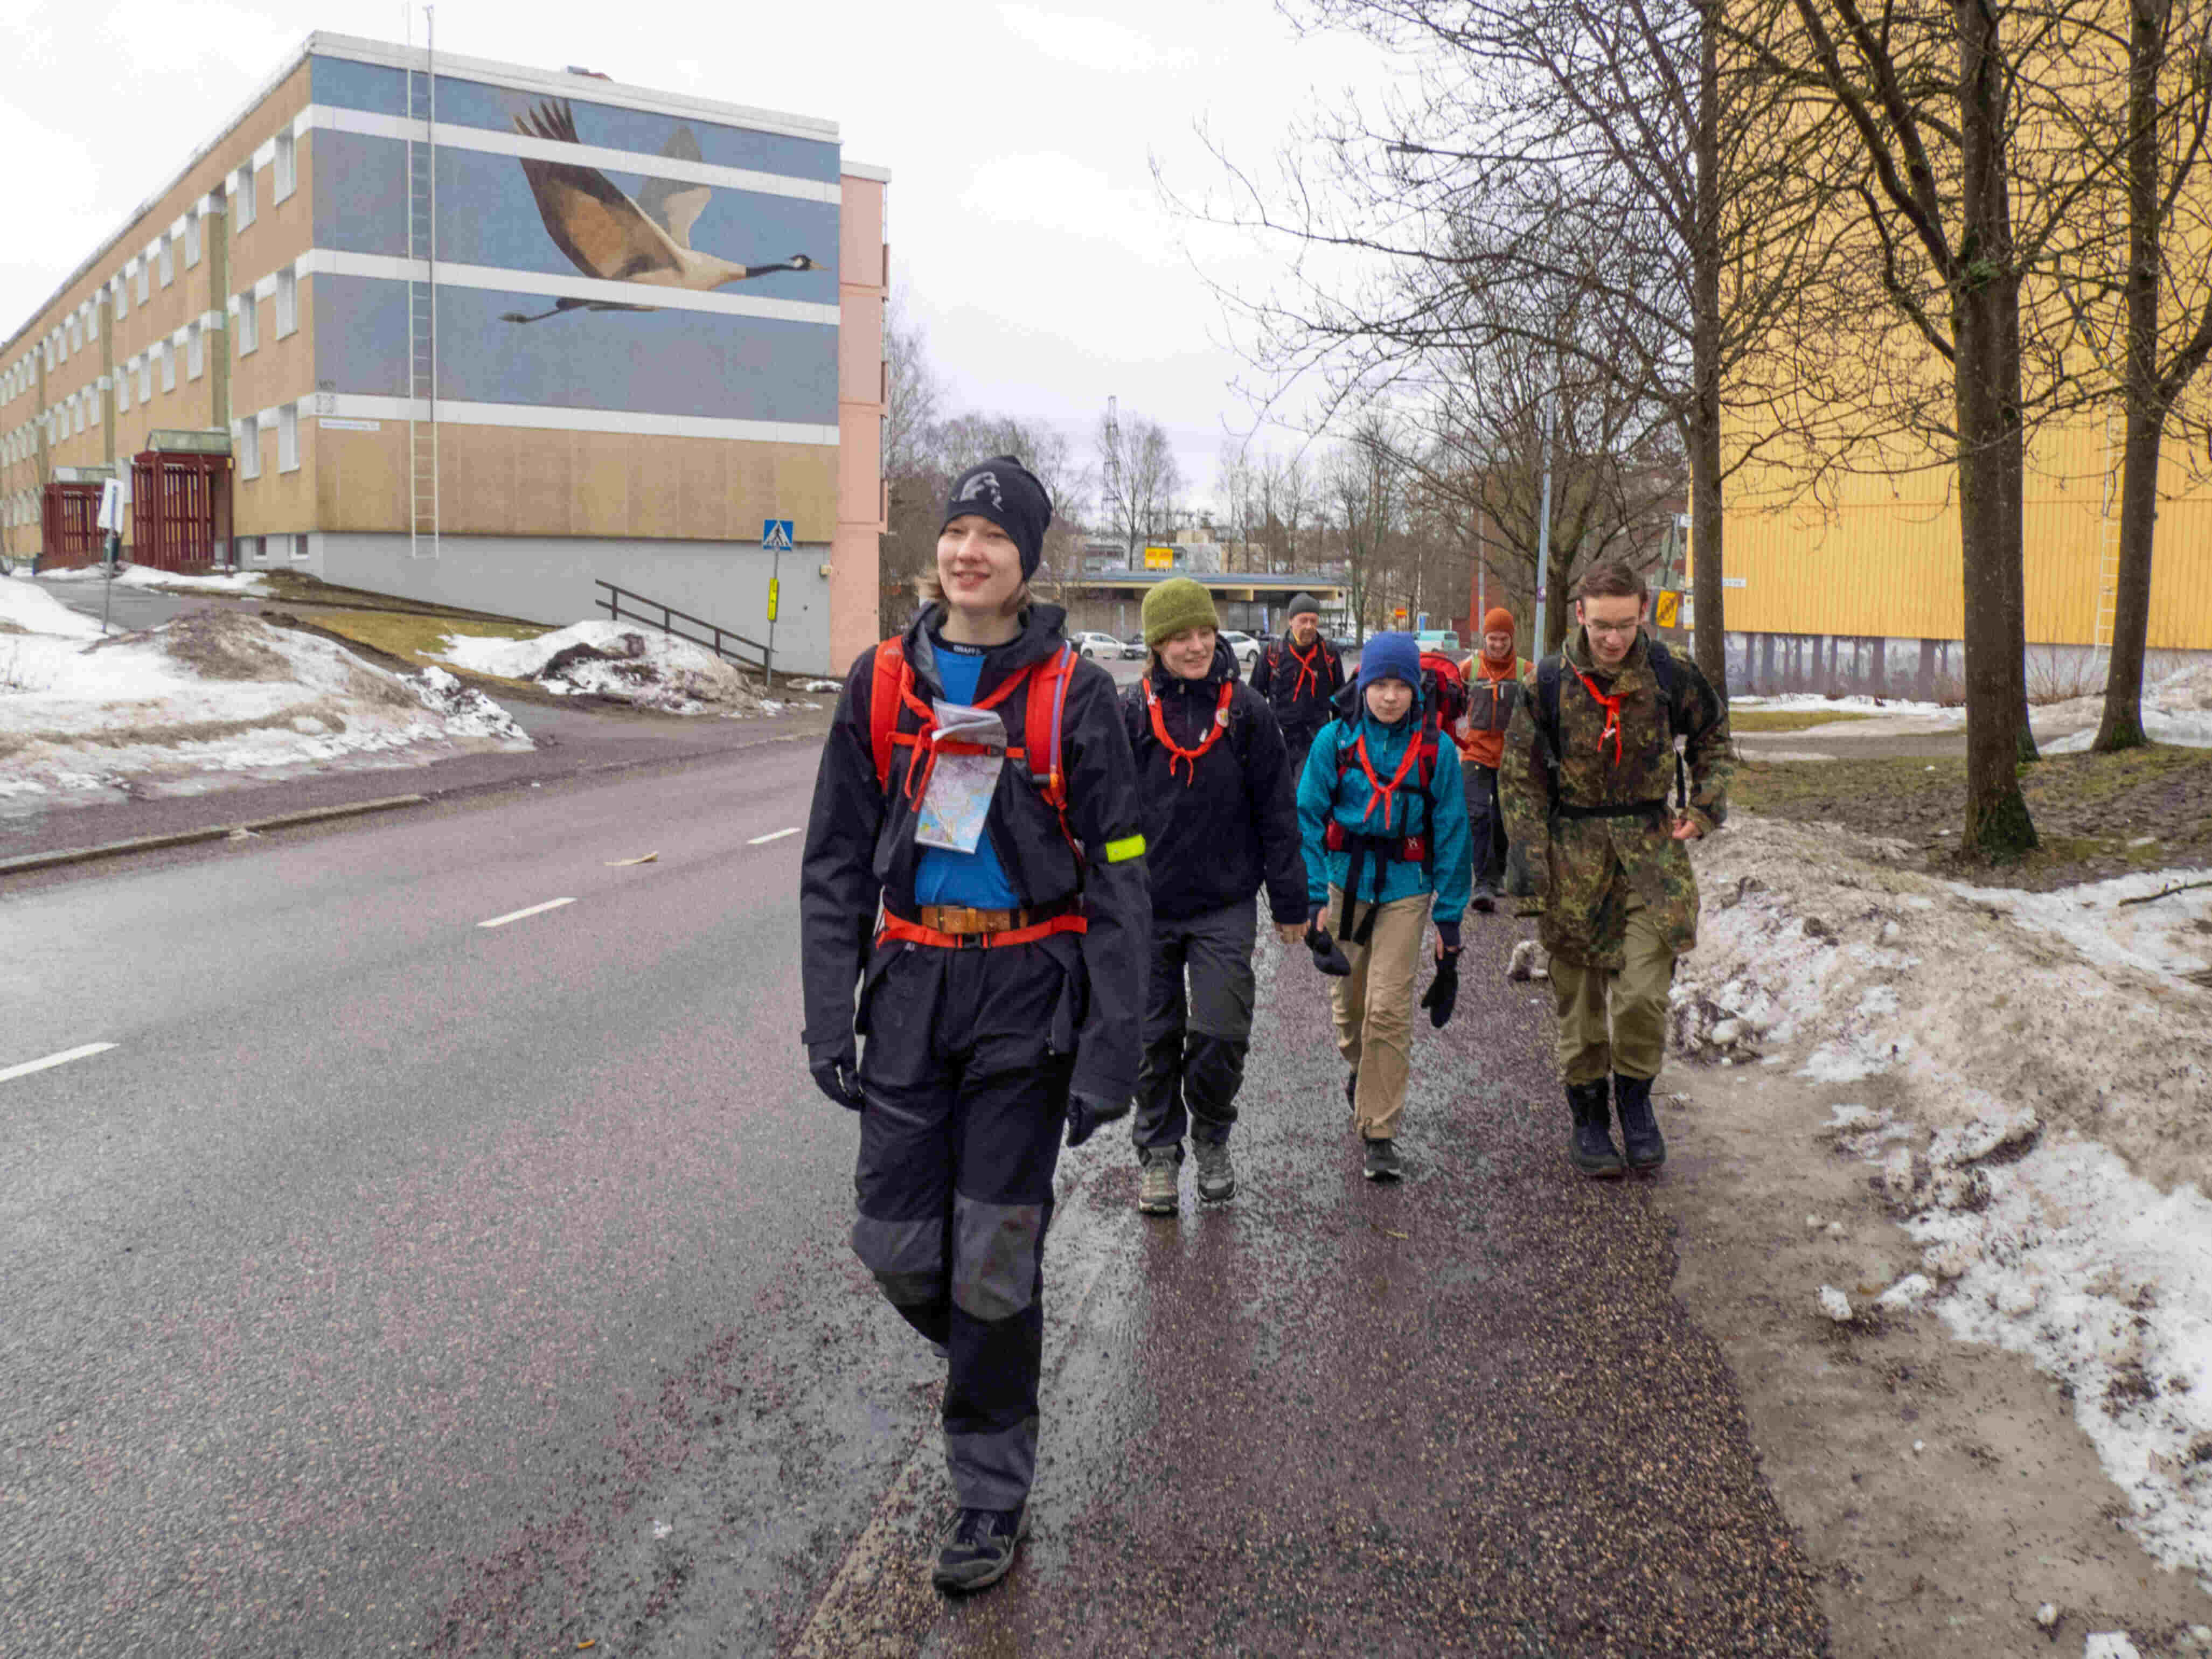
\includegraphics[width=\linewidth]{assets/nahkaliljavantaa}

	Pian oltiinkin jo Vantaan puolella, kun reittimestari ohjasi vaeltajia
	ansiokkaasti Vesalan läpi yli Keihäsrinteen liukkaiden mäkien. Vantaan
	kaupunginosista reitin aikana koettiin kaksi: Rajakylä ja Länsimäki,
	joista – jos ei muuta – saatiin kerättyä muutama silta lisää, ja joista
	ensimmäisessä sijaitsi reitin pohjoisin piste.

	Reitti kaartui jyrkästi etelään ja ensimmäinen poikkeama suunnitellulta
	reitiltä tehtiin tietoisesti \textbf{kello 9.40}, kun vaihdettiin
	puolta Länsimäentiellä pitkin Juoksuhaudanpuiston ylikulkukäytävää
	viheralueelle, jonka läpi menevä ulkoilutie oli varsin kostea.
	Kuntopolku aiheutti hilpeyttä osassa osallistujista, koska tie ei ollut
	kovinkaan pitkä. Vaelluksen ensimmäinen suunnittelematon poikkeama
	tehtiin \textbf{kello 9.52}, kun Keilapolun alikulkukäytävä ylitettiin
	kahteen kertaan.

	Pian oltiinkin takaisin Helsingin puolella. Likimain Mellunmäentien ja
	Naulakalliontien risteyksessä Tanguy huudahti ensimmäisen viiden
	kilometrin merkin, minkä jälkeen alettiin etsiä soveltuvaa
	taukopaikkaa. Sellainen löydettiin Naulakallionpuistosta, jossa
	pysähdyttiin evästämään ja ottamaan ryhmäkuva. Tauko päättyi
	\textbf{kello 10.14}.

	\vspace*{0.32cm}
	\noindent\includegraphics[width=\linewidth]{assets/nahkaliljaryhmä}

	Reitti jatkui kaakkoon, seisahdus Itäväylällä ja jo
	Linnavuorenpuistossa \textbf{kello 10.38} alettiin arpoa, kuinka monen
	sillan yli sitä oli mentykään. Kävelyalusta oli talven aikana
	ladutettu, eli tiiviiksi tampattua nyt jo märkää ja jäätynyttä lunta.
	Onneksi tie Vartiokylänlahden toisella puolella oli paljon
	käveltävämmässä kunnossa. Taktisesti seuraava tauko pidettiin jo
	Vuosaaren sillan kupeessa odottaen seuraavaa etappia läpi Puotilan,
	Marjaniemen ja Roihuvuoren. Eväät maistuivat hyvin eikä kenenkään askel
	painanut tavanomaista enempää. Tauolla pohdittiin läheisen rakennuksen
	seinässä ollutta "vSv"-lyhennettä. (Toim. huom. oikea vastaus olisi
	ollut Vuosillan Veneilijät.)

	Vuosaaren sillalla ihmeteltiin uhkarohkeaa pilkkiosastoa, joka
	keväisestä maaliskuun lauantaista huolimatta eteni Vartiokylänlahdella
	\textbf{kello 11.16}. Mikko kuvasi toimintaa nasevasti yhdellä sanalla:
	"Luonnonvalinta." Jo useamman kerran reitti ohitti kaupungin hienot
	opaskyltit itäisestä rantareitistä, joka – nyt jälkikäteen ajatellen –
	voisi olla ihan hauska retki sekin.

	Marjaniemessä ihmetystä aiheutti Vanhalla Koivuniementiellä olleen
	asuinrakennuksen voimakkaasti heijastavat seinäpaneelit, joista
	varmasti naapurit olivat mielissään. Leikkipuisto Iso-Antin nimen
	alkuperää yritettiin tavata Tapio Rautavaaran sanoin "Isontalon Antti
	ja Rannanjärvi / Ne jutteli kaharen kesken". Todennäköisempää lienee
	kuitenkin, että leikkipuisto on saanut nimensä viereisestä Ison-Antin
	tiestä, josta Helsingin kadunnimet (1992) osaa kertoa seuraavaa:

	"Ison-Antin tie — Stor-Andersvägen, 1949. Nimi käytössä jo ennen 1946
	asussa Antintie — Andersvägen, Marjaniemen huvilayhdyskunnan
	perustaja-asukkaihin kuuluneen rakennusmestari Antti Hongiston mukaan,
	jota kutsuttu »Isoksi Antiksi»."

	Nimistökysymyksen jälkeen reitti jatkui länteen. Roihuvuoren rajalla
	alkoivat kuulua ensimmäiset merkit kävelyn aiheuttamasta rasituksesta,
	kun joidenkin vaeltajien jalat alkoivat painaa. Jyrkkä käännös etelään
	ja Tammisalon kanavan yli, Pyörökiventien varressa muuan mies lapioiden
	levitti lunta pihallaan ja pyysi seuruetta talkoisiin. Mikko kieltäytyi
	kohteliaasti kertoen miehelle matkaa olevan jäljellä vielä
	kolmekymmentäviisi kilometriä.

	Likimain viidentoista kilometrin tauko osui Kiiltomadonpuistoon – josta
	kertovasta kyltistä Toivon oli saatava kuva – \textbf{kello 12.22},
	jolloin osa seurueesta vaihtoi jalkaansa kuivat sukat ja kevensi
	varustustaan pilvien välistä pilkottelevan auringon lämmittävän
	vaikutuksen takia.

	Tauon jälkeen jatkettiin vielä etelään, kunnes saavutettiin reitin
	eteläisin piste, Kettu Repolaisen puisto, jossa reitti teki
	u-käännöksen palaten mantereen puolelle Laajasalon siltaa pitkin.
	Seuraava tauko tulikin tavanomaista nopeammin reilu kolme kilometriä
	myöhemmin, kun seurue pysähtyi istumaan Laivalahdenkaaren ja
	Kerttulinkujan kulmassa kasvavan hevoskastanjan alle noin \textbf{kello
	13.15}. Tauko kulki nimellä "Piolimatkankrouvi", vaikka todellisuudessa
	ei sitä ihan vielä ollutkaan. Tulipa seuruetta ihmettelmään muuan
	rouva, joka uteliaisuuttaan tuli kysymään, mistä lippukunnasta
	vaeltajat olivat.

	Nopea taktinen tauko Hitsaajankadun Picnic-kahvilassa ja pian oltiin
	matkalla kohti kaupungin keskustaa. Varustusta lisättiin ennen
	Naurissaaren siltaa kolean länsituulen viilentäen vaeltajia. Läpi
	Kulosaaren, seuraava tauko ja seuraava rouva osuivat Mustikkamaalle
	\textbf{kello 14.28}. Kruunusiltojen työmaata ihmeteltiin ylitettäessä
	Isoisänsiltaa, josta reitti yhtyikin vuoden 2022 Hiipivä Haamu
	-salapoliisikilpailun ennakkotehtävien kaupunkikierrokseen.

	\vspace*{0.16cm}
	\noindent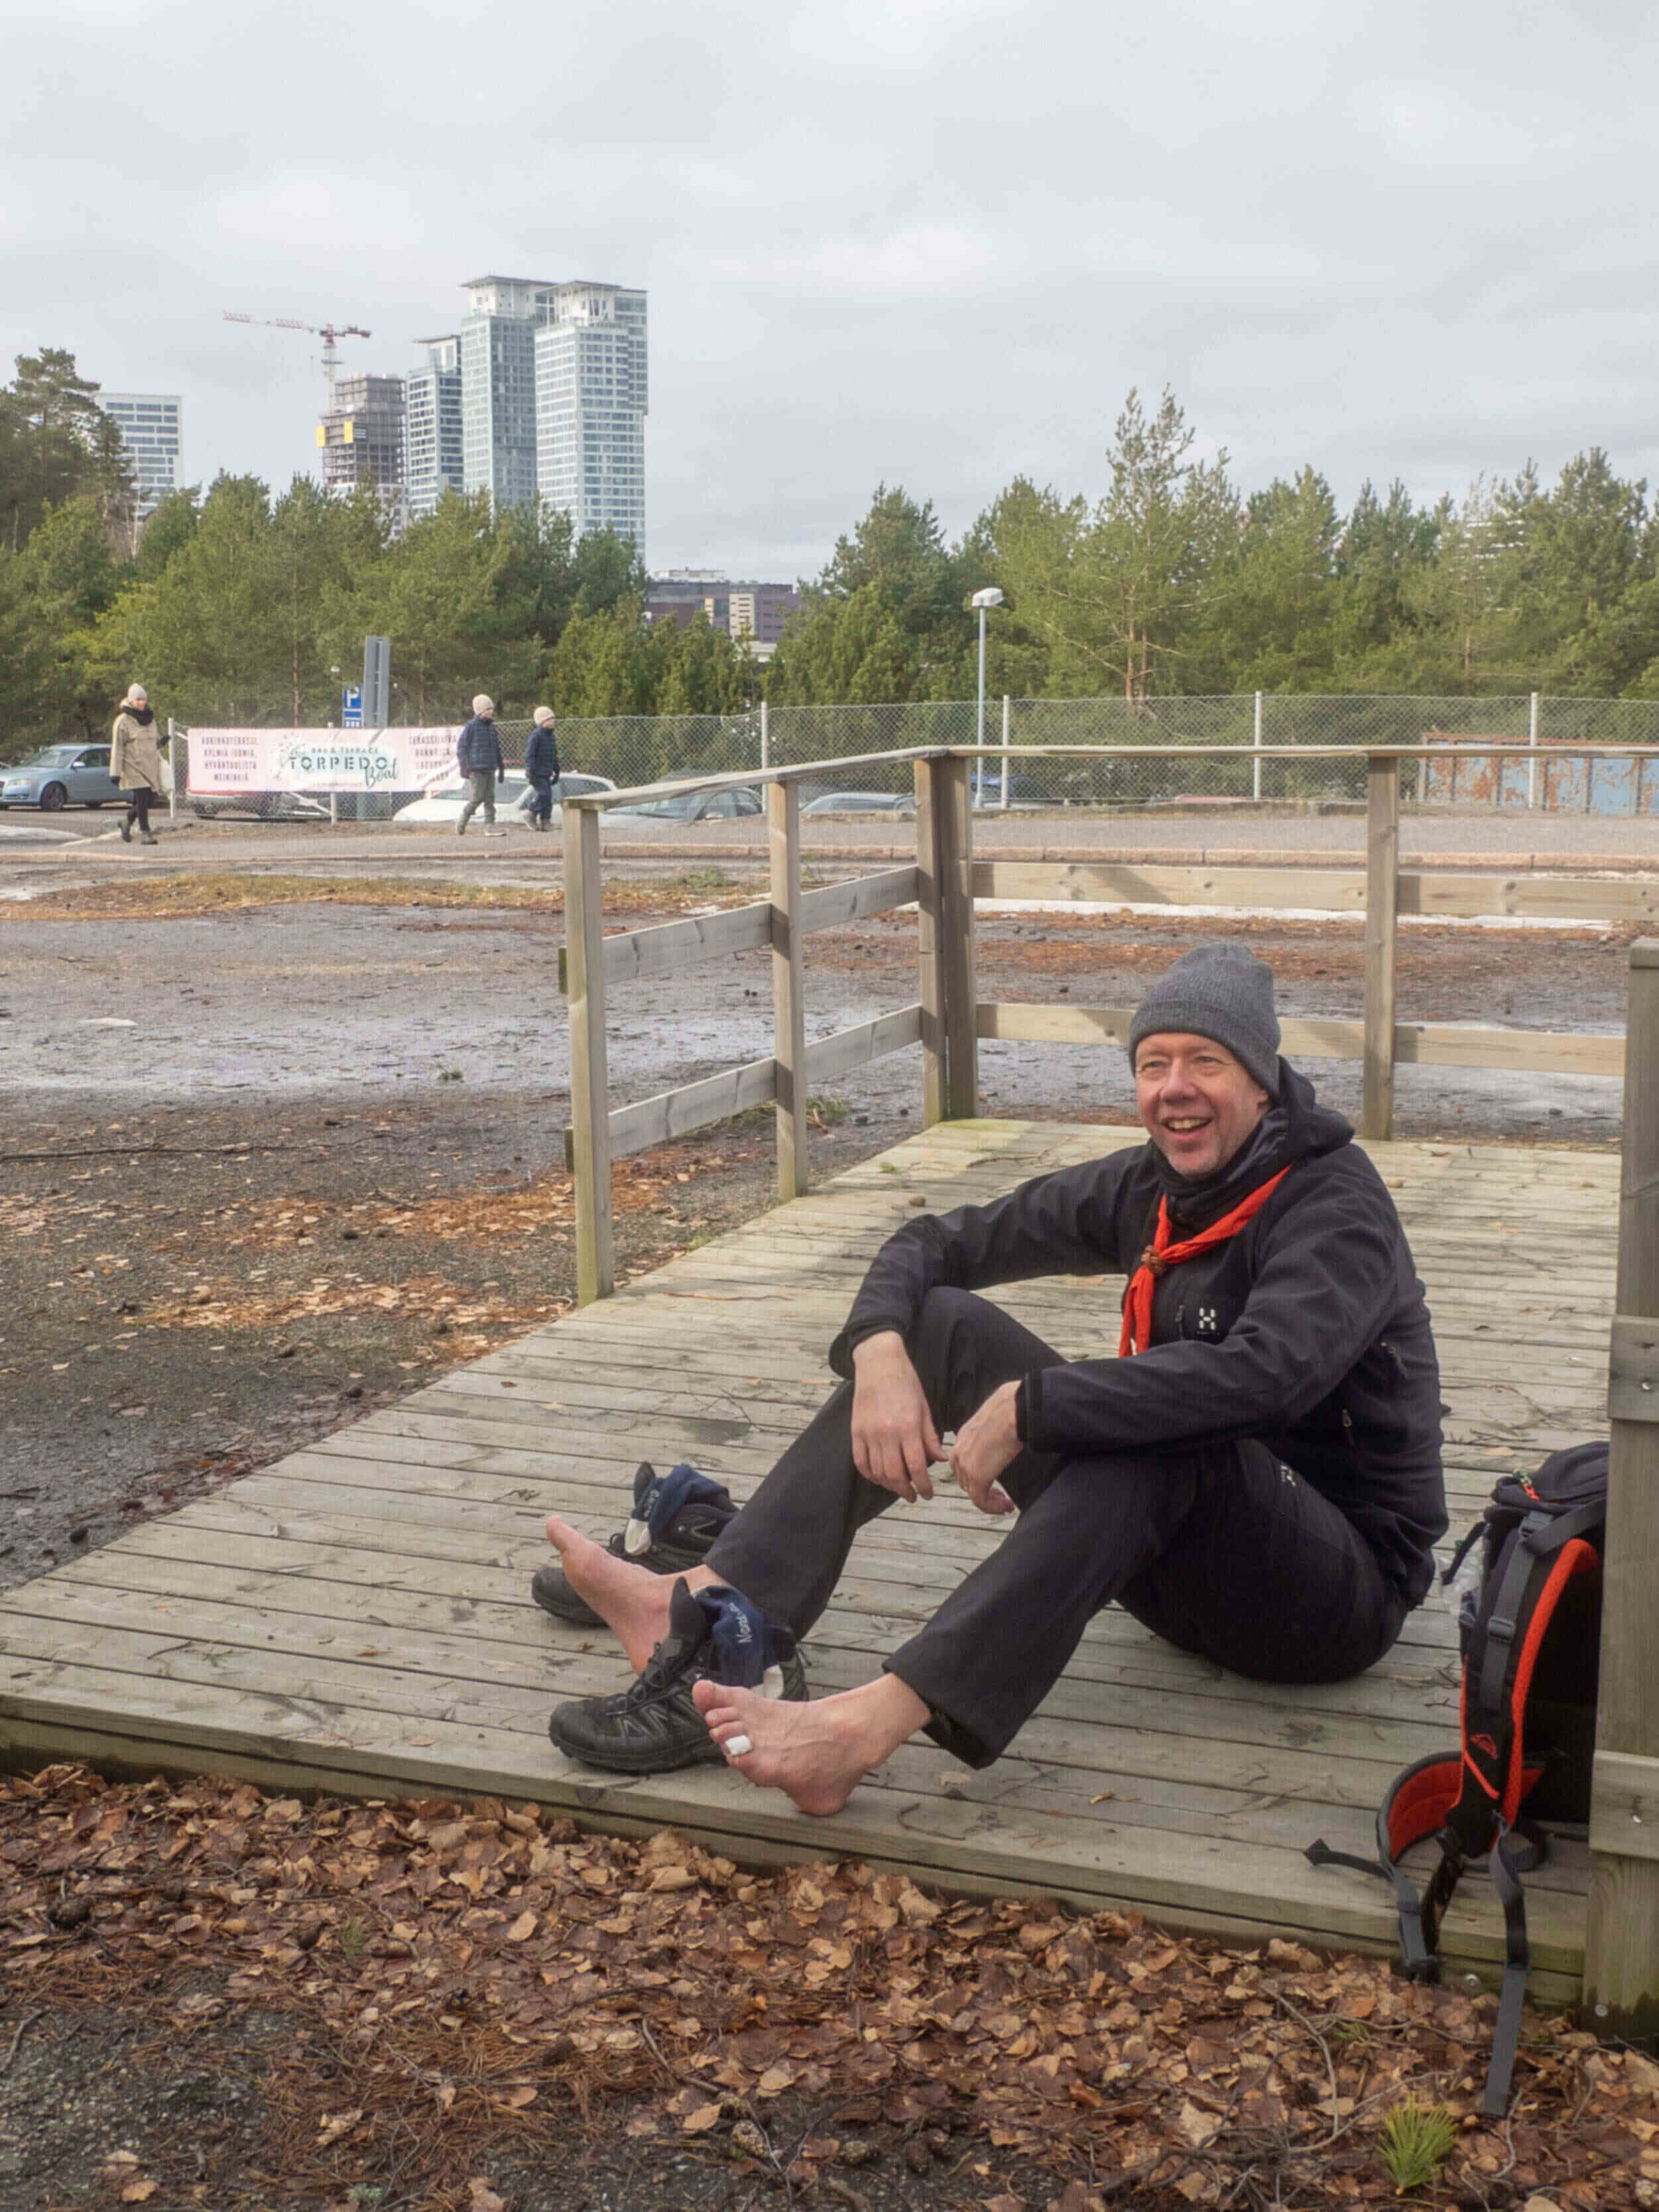
\includegraphics[width=\linewidth]{assets/nahkaliljamikko}

	\vspace*{0.16cm}
	\noindent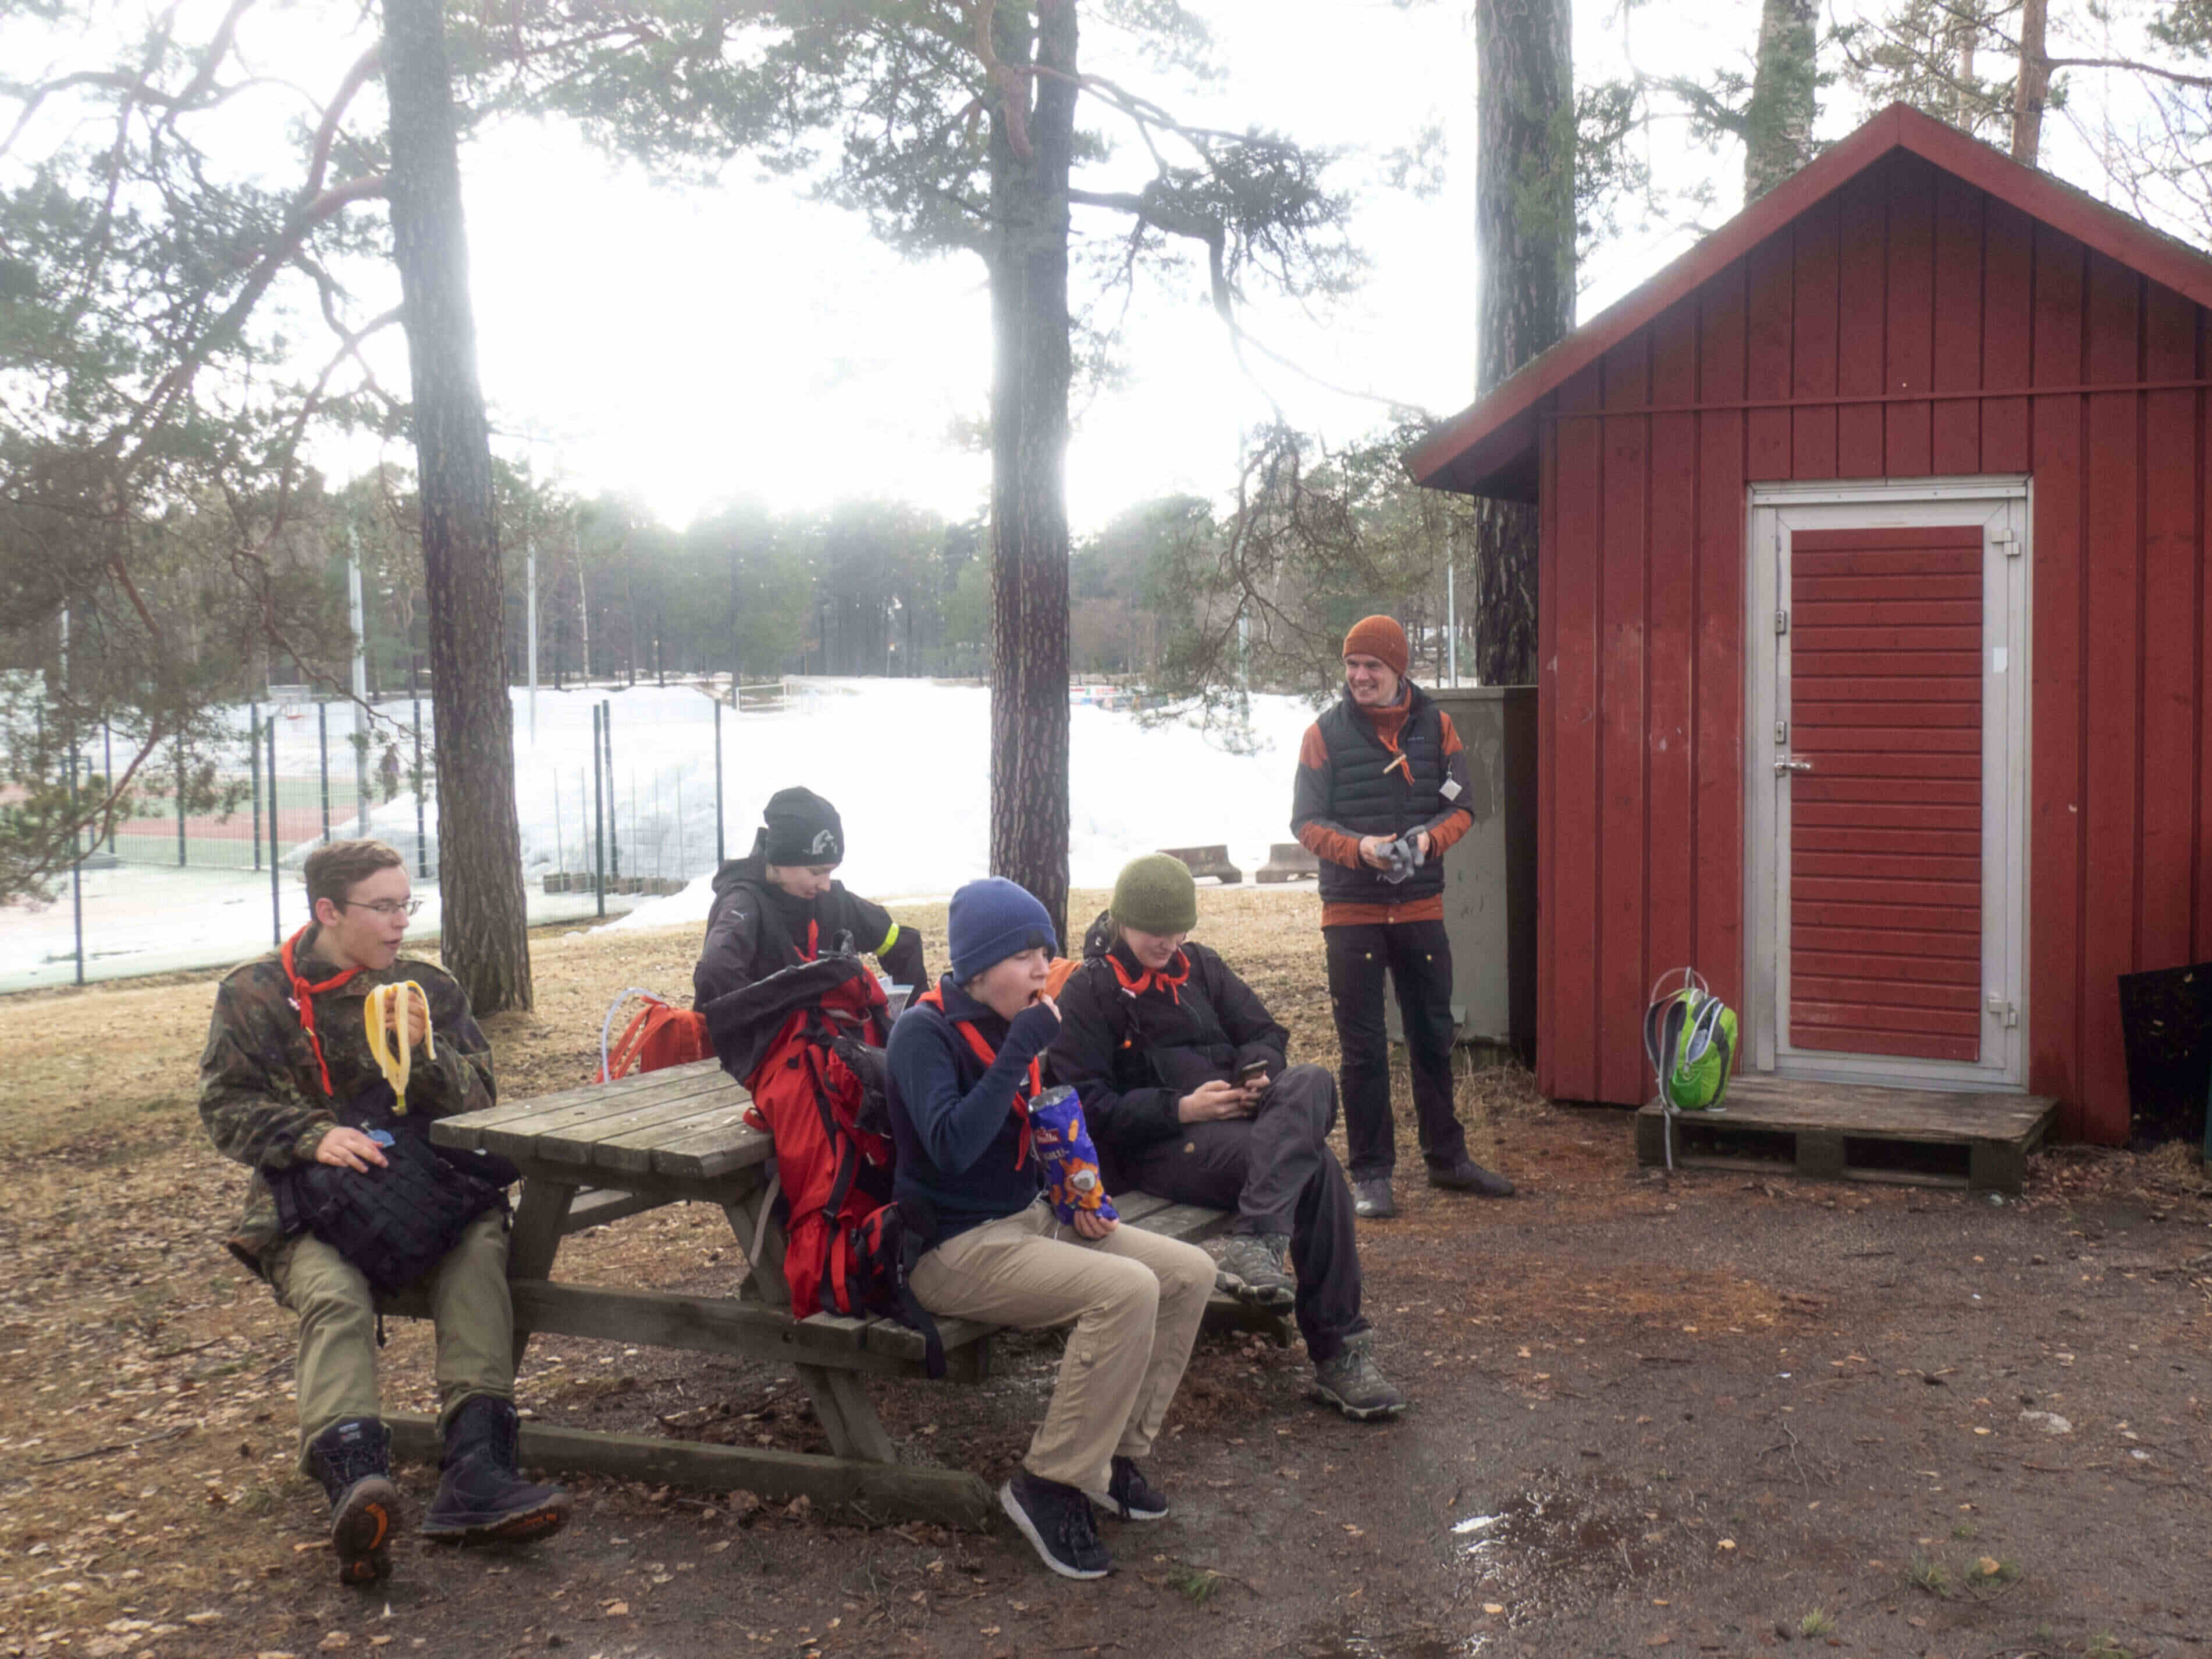
\includegraphics[width=\linewidth]{assets/nahkaliljamustikkamaa}

	\noindent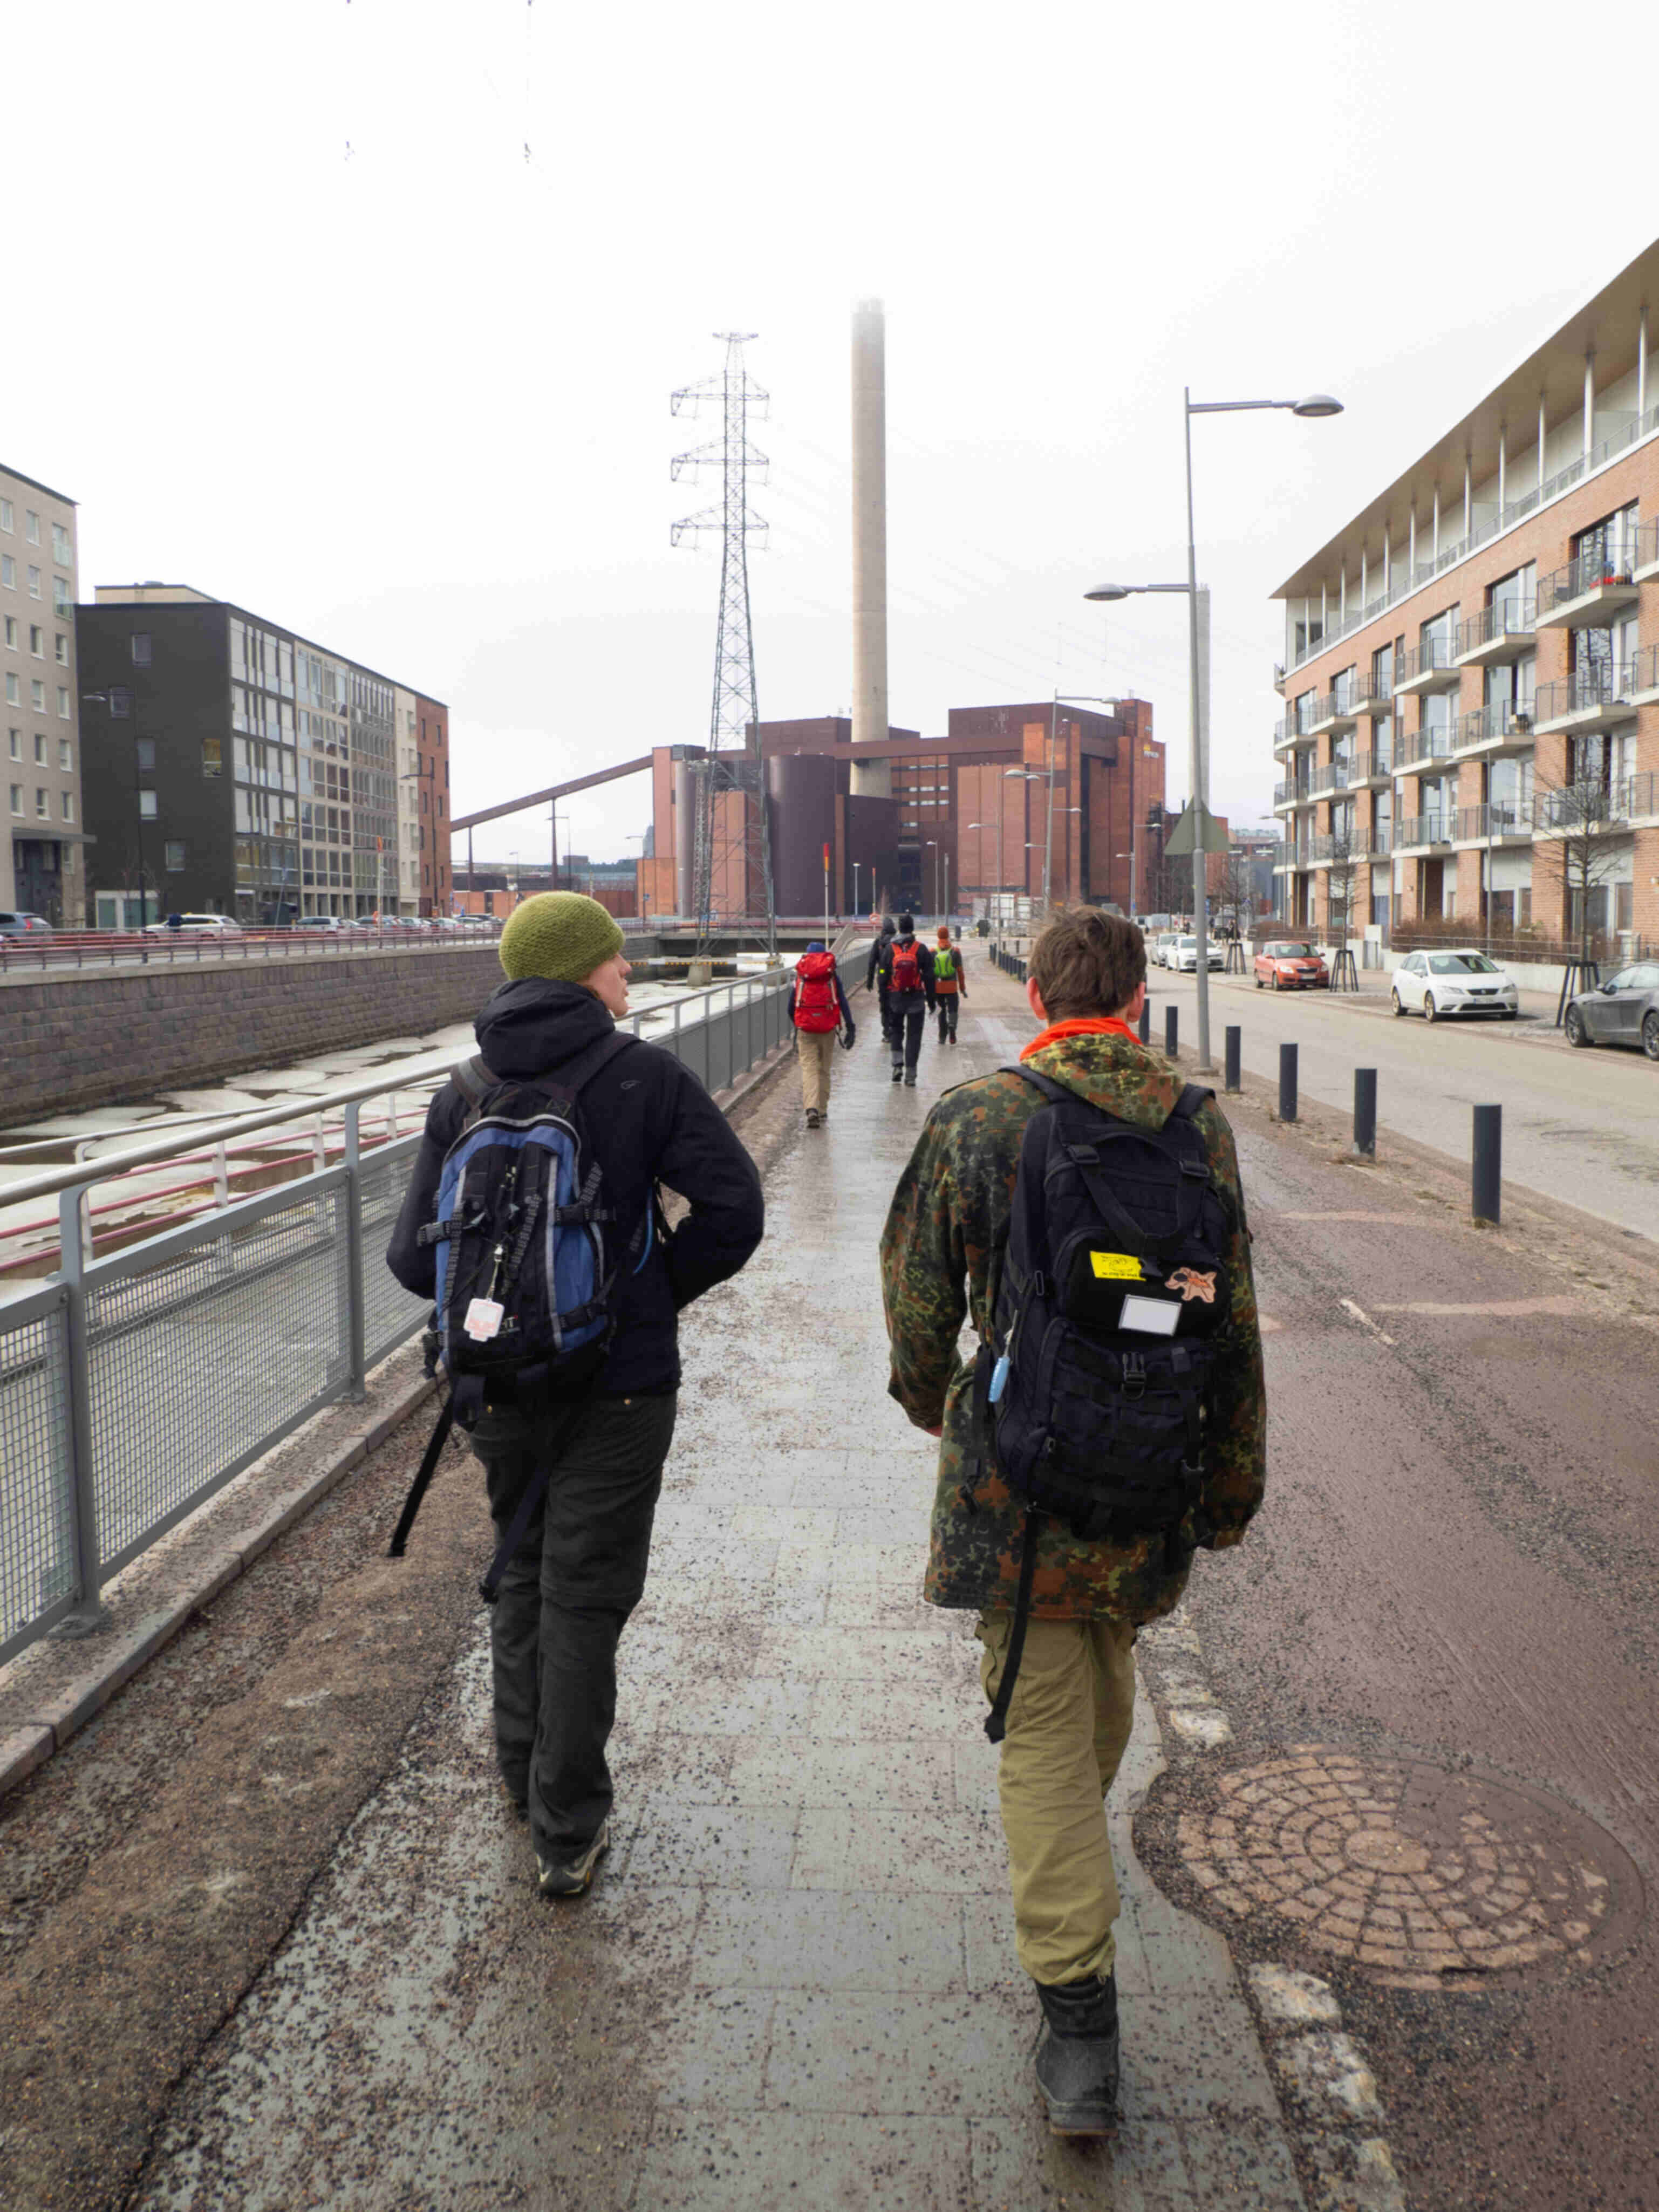
\includegraphics[width=\linewidth]{assets/nahkaliljakalasatama}

	Hakaniemen läpi päästiin juuri ja juuri jo mainitun liikennehankkeen
	työmaiden välistä pujotellen. Seureen etenemisvauhtia kuvasi hyvin
	Mikon kommentti, kuinka kukaan ei ollut vielä onnistunut vaeltajia
	ohittamaan. Kaisantunneli ei ollut ehtinyt vielä valmistua, mutta
	onneksi Linnunlaulun silta sai seurueen junaratojen länsipuolelle.
	Hakasalmen puistossa Töölönlahden rannalla Janne ja Tanguy nauttivat
	mämmiä \textbf{kello 15.44}. Kuivat sukat jalkaan ja vaellus jatkui.
	Jalkojen lisäksi myös nälkä alkoi painaa osaa vaeltajista. Linnuntietä
	maaliin oli yli kymmenen ja puoli kilometriä, mikä tarkoitti sitä, että
	vaadittu neljäkymmentä kilometriä tultaisiin todennäköisesti
	ylittämään.

	Töölönlahden kierron jälkeen suunta otettiin kohti maalia. Arvottiin,
	jahka oikaistaisiin takaisin Itäväylän vartta, mutta reittimestari
	pysyi vankasti reittisuunnitelmassaan. Sturenkatu ei tarjonnut
	erityisen kiinnostavaa maisemaa kävelylle, mutta Vallilan paahtimo
	herätti muistoja. Mäkelänkadun Subway tarjosi taktisen pysähdyksen,
	josta vauhtia sen enempää hidastamatta jatkettiin Arabianrantaan.

	Toukolan rantapuiston Laituri-ympäristötaideteos – tarkemmin,
	kuvataiteilija Merja Salosen laituri, jossa "näkyvät lapsuusmuistona
	mummolan järven hiekkapohjan aaltokuviot" – tarjosi seurueelle
	hengähdystauon ja istumapaikan \textbf{kello 17.01}. Tauon aikana muuan
	Toimen Tytöt -partiolippukunnan jäsen tuli ihmettelemään rusakoiden
	oransseja huiveja ja kertomaan, kuinka heidän partio-ohjelmansa
	riihityksessä oltiin hiihdetty kymmeniä kilometrejä vaikeakulkuisen
	puistikon läpi. (Toim. huom. TT muutti Töölöstä Arabianrantaan vuonna
	2008.) Tauko päättyi \textbf{kello 17.22}.

	Arvioitaessa Vanhankaupunginkosken ylitystä päädyttiin lyhimpään ja
	nopeimpaan ratkaisuun ylitettävien siltojen lukumäärän kustannuksella.
	Tässä vaiheessa vaeltajien välimatkat jo kasvoivat merkittävästi
	toisten jalkojen painaessa enemmän kuin toisten.

	Viikinportinkadun risteyksessä arvioitiin uudelleen nopeinta
	mahdollista reittiä maaliin, mutta jälleen reittimestari pysyi vankasti
	etukäteen valmistellussa reitissä. Tähän mennessä alkuperäinen
	taukostrategia oli riekaleina niin taukojen välimatkojen kuin niiden
	kestonkin suhteen; seuraava tauko pidettiin Viikintien varressa
	luonnonsuojelualueen kulmassa \textbf{kello 18.02}, jossa levättiin jo
	kevyenliikenteenväylällä maaten.

	Seurasi reitin tylsin osuus, Viikin suora, jolla itse kukin tunsi tai
	ei tuntenut jaloissaan aivan uusia tuntemuksia. Viikintieltä käänyttiin
	kohti Hallainvuorta ja Ilmolanraitilla pidettiin tauko \textbf{kello
	18.35}. Osallistujien mittarit näyttivät tässä vaiheessa neljänkymmenen
	kilometrin jo täyttyneen. Lippukunnan kolo oli jo kivenheiton päässä.
	Liukastelua vanhalla latupohjalla ja pian oltiin jo tutussa ja
	turvallisessa Kivikossa, kun seurue ylitti Kehä I:n Viikinpuistonsiltaa
	pitkin.

	Kivikon puolella pohdittiin, sikäli mikäli maaliin olisi välttämätöntä
	kaikkien kävellä, koska määritelty matka oli mitä todennäköisimmin jo
	saatu täyteen. Niinpä Elias erkani seurueesta kotimatkalle
	Kivikonlaidan varrella \textbf{kello 18.59}, Tanguy ja Toivo jäivät
	Kivijatatien bussipysäkille \textbf{kello 19.06} ja Leon autokyyti otti
	hänet mukaansa Panosaukion tuntumasta \textbf{kello 19.09}.

	Jäljelle jääneet vaeltajat Ahti, Janne ja Mikko kävelivät maaliin asti,
	jossa he olivat reittimestarin kellon mukaan \textbf{kello 19.32}. Koko
	matkan pituudeksi tuli tarkistusmittauksen jälkeen reilu
	neljäkymmentäkolme kilometriä, mikä tarkoitti noin 4,2 kilometrin
	tuntivauhtia – todella haipakkaa siis. Punaisen nahkaliljan
	viisikymmentä kilometriä ei siis ole haaste eikä mikään!

	Ilmatieteen laitoksen Kumpulan havaintoasemalla merkittiin
	vaelluspäivän sääksi puolipilvisestä pilviseen, lämpötila 2–5 astetta,
	länsituulta 3–7 metriä sekunnissa ja ilmankosteus 77–93 prosenttia –
	mitä erinomaisin nahkaliljakeli, sanoisin!\\

	\vspace*{0.50cm}

	\raggedleft Toimittaja: Janne Suomalainen\\
	\vspace*{0.10cm}
	\raggedleft Kuvat: Tanguy Gérôme

\end{multicols}

\begin{center}
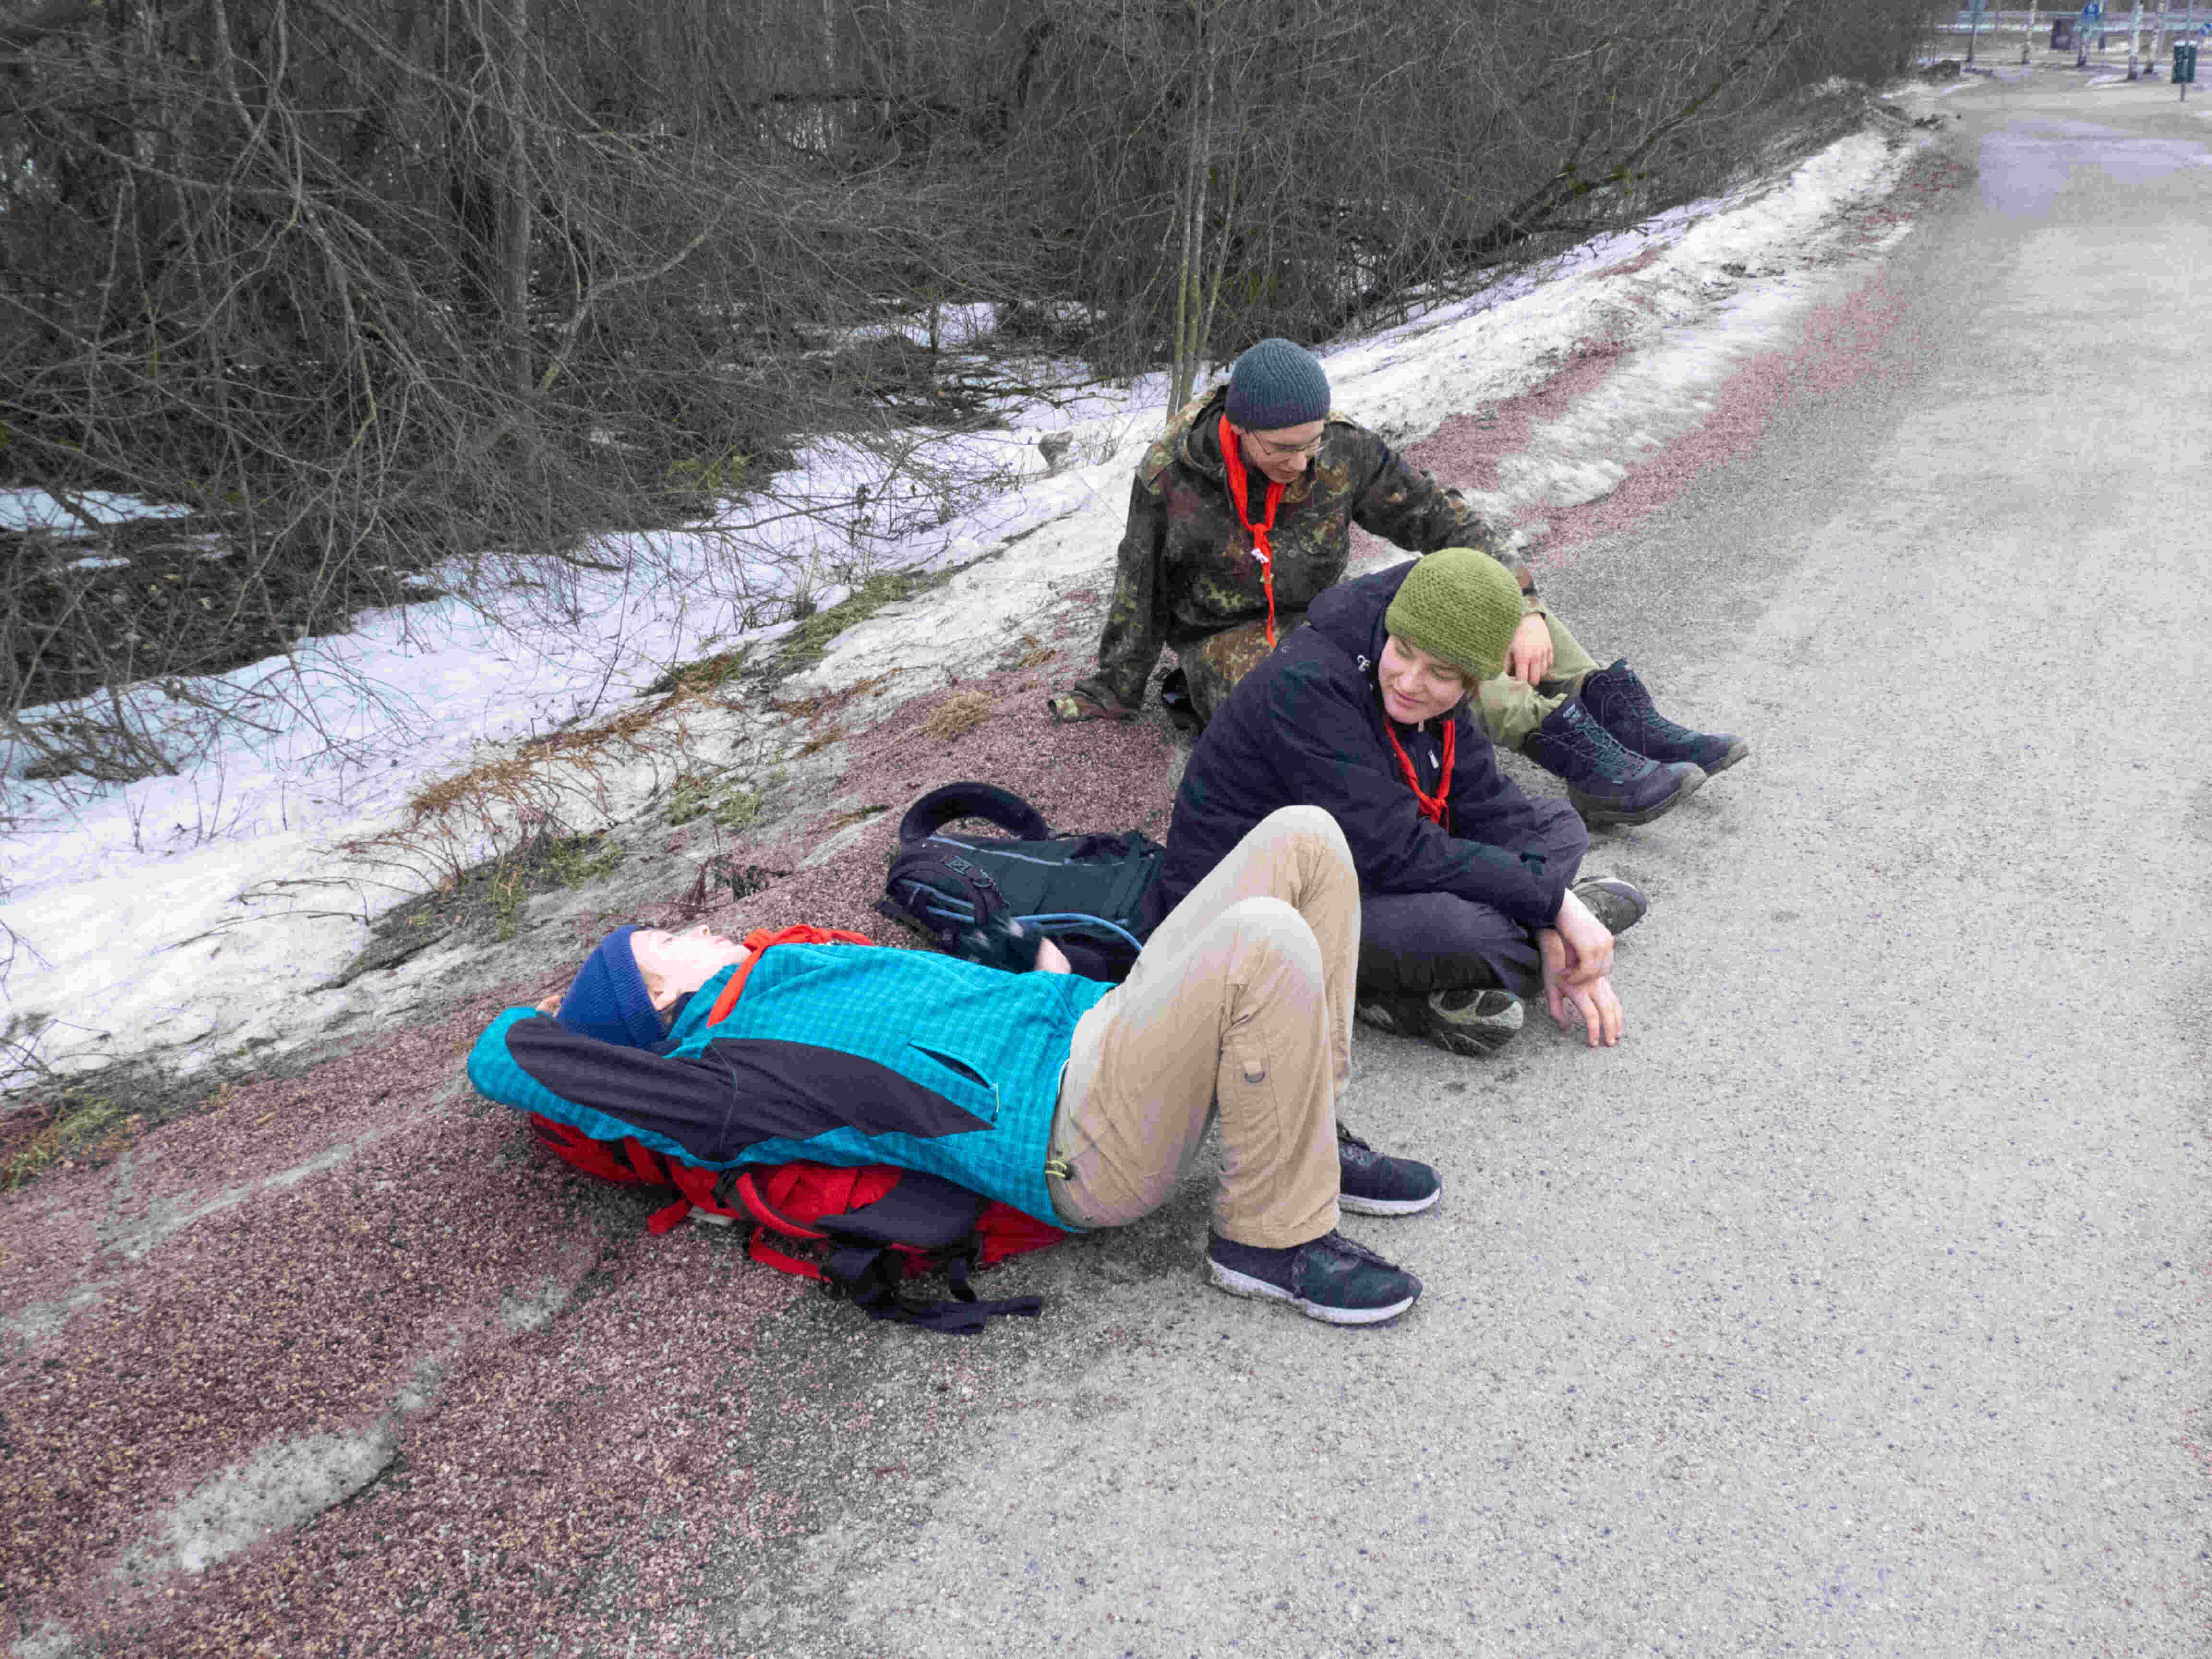
\includegraphics[width=0.65\linewidth]{assets/nahkaliljaviikki}
\end{center}

Lopuksi, tässä on jokaisen osallistujan kolmen sanan tiivistelmä.
Valitettavasti, päätoimittaja sekoitti hänen muistiinpanonsa.
Teillä on tehtävä: kuka sanoi mitä.

\begin{center}
	\begin{tabular}{ |c||ccc||c| }
		\hline
		Ahti & a. & & 1. & hauska hyvä sää \\
		\hline
		Elias & b. & & 2. & jalat irtoavat pois \\
		\hline
		Janne & c. & & 3. & kipu kärsimys ruoka \\
		\hline
		Leo & d. & & 4. & minä pidän kävely \\
		\hline
		Mikko & e. & & 5. & mulla on nälkä \\
		\hline
		Tanguy & f. & & 6. & oli hauska aloituksessa \\
		\hline
		Toivo & g. & & 7. & optimaalinen reipas keväinen \\
		\hline

		% Ahti & a. & & 1. & hauska & hyvä & sää \\
		% \hline
		% Elias & b. & & 2. & jalat & irtoavat & pois \\
		% \hline
		% Janne & c. & & 3. & kipu & kärsimys & ruoka \\
		% \hline
		% Leo & d. & & 4. & minä & pidän & kävely \\
		% \hline
		% Mikko & e. & & 5. & mulla & on & nälkä \\
		% \hline
		% Tanguy & f. & & 6. & oli & hauska & aloituksessa \\
		% \hline
		% Toivo & g. & & 7. & optimaalinen & reipas & keväinen \\
		% \hline

		% Ahti & minä & pidän & kävely \\
		% \hline
		% Elias & mulla & on & nälkä \\
		% \hline
		% Janne & optimaalinen & reipas & keväinen \\
		% \hline
		% Leo & kipu & kärsimys & ruoka \\
		% \hline
		% Mikko & hauska & hyvä & sää \\
		% \hline
		% Tanguy & oli & hauska & aloituksessa \\
		% \hline
		% Toivo & jalat & irtoavat & pois \\
		% \hline

		% Ahti & minä pidän kävely \\
		% \hline
		% Elias & mulla on nälkä \\
		% \hline
		% Janne & optimaalinen reipas keväinen \\
		% \hline
		% Leo & kipu kärsymys ruoka \\
		% \hline
		% Mikko & hauska hyvä sää \\
		% \hline
		% Tanguy & oli hauska aloituksessa \\
		% \hline
		% Toivo & jalat irtoavat pois \\
		% \hline
	\end{tabular}
\end{center}

